%!TeX root=../Dissertation.tex
%!TeX bibfile=./introduction.bib

\chapter{Introduction}
\section{Summary of the Current Situation}
\label{CurrentSituation}
Within computer networking, and computing as a whole, we tend to move through paradigms. Generally, there is a set way of doing things and eventually there are breakthroughs that shift that standard. One such paradigm is the use and reliance of Virtual Machines in the hosting of servers. As written by \citet{VirtualNetworkingInTheFuture}, ``Virtualization has rapidly become a go-to technology for increasing efficiency in the data center.''. Ameen and Hamo were right when they wrote this in 2013 and more and more server infrastructure has moved to virtualisation since. If we look at uptake of virtualised networking, servers and storage more recently, we see can see that virtualisation has become one of the de-facto solutions for server management. \citet{Spiceworks} found in ``The 2020 State of Virtualization Technology'' report that 92\% of the companies that they surveyed already used server virtualisation, with a further 5\%  planning on adopting it within two years of that date \citep{Spiceworks}. Some of the main reasons for this extremely high adoption are: savings in power and hardware (One physical machine can support multiple servers) and Logical Resource Consolidation \citep{LetsGetVirtual}. These savings however, don't come at no cost. One of the main stresses on any virtualised server infrastructure is the high resource usage that comes with hosting more than one server-based service on one physical machine. As server tasks become more strenuous, or when entirely new services need to be added to an already existing infrastructure, we can find that hardware (such as memory and CPU usage) becomes overwhelmed \citep{LetsGetVirtual}. As the tech world moves forward, the infrastructure that supports that tech within organisations needs to do so too. This is why we are starting to see a large number of organisations moving to cloud-based infrastructure, or taking the leap to invest in upgraded server hardware, that can withstand the large workloads required for some modern-day server loads. These solutions however, come with their own problems and negate the key reasons that these organisations moved to virtualisation in the first place. Cloud-based solutions, whilst being able to take the onus away from an organisations infrastructure team, can also result in costly hosting fees, not to mention the fact that cloud services often can't be used in place of some internal network components, such as DHCP and internal DNS servers. The other solution; upgrading hardware, again misses the mark and undermines the reasoning for why virtualisation was implemented in the first place. As already discussed, virtualisation is preferred because it can save money on costly server infrastructure. Instead of having to purchase (and power) several physical machines, you have one powerful machine that can support all the same services. When we reach the ceiling in terms of output from that sole machine, an upgrade seems inviable, but at this point, how much money was actually saved? Once you factor in the extra overhead that running a virtual machine introduces as a result of Virtual Machine and OS virtualisation resource usage (Figure \ref{fig:VirtualisationDiagram}), we start to see that Virtualisation might not be the perfect solution it once was.


\fbox{\parbox{\dimexpr\linewidth-2\fboxsep-2\fboxrule\relax}{\centering For reference only, Figure \ref{fig:VirtualisationDiagram} \\ 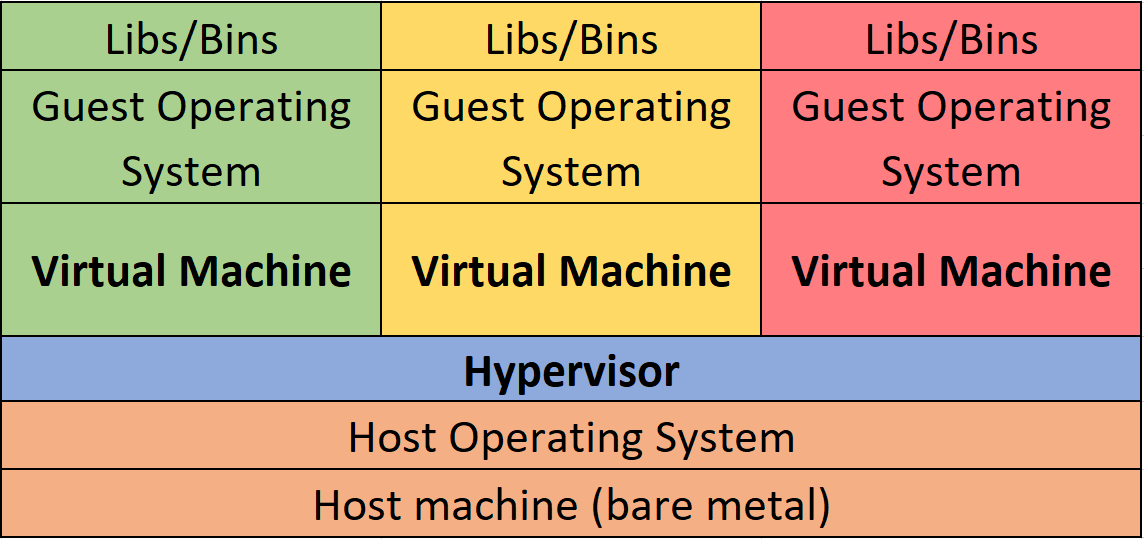
\includegraphics[width=0.9\textwidth]{./analysis/VMdiagram.PNG}}}

\section{A New Contender: Containers}
One possible solution to this problem, is instead of upgrading hardware, organisations simply remove the Virtual Machine and virtualised OS components, along with their resource utilisation, whilst keeping the core functionality of the servers that they host intact, as shown in Figure \ref{fig:ContainerDiagram}. This is where containerisation comes into play. Containerisation, removes the need to virtualise a whole Operating System for each virtual machine, instead ingratiating with the host machine's Operating System directly with what is being run in the container, whilst keeping each container separated logically. These containers can still interface with real networks in much the same way that Virtual Machines do but also reduce the overheads and as result, the hardware resource utilisation dramatically. This allows SME's and other organisations currently using Virtualisation to squeeze more performance out of their already existing hardware without having to do costly upgrades to hardware.

\fbox{\parbox{\dimexpr\linewidth-2\fboxsep-2\fboxrule\relax}{\centering For reference only, Figure \ref{fig:ContainerDiagram} \\ \includegraphics[width=0.9\textwidth]{./analysis/Condiagram.PNG}}}

The research in this project report aims to contribute to this possible paradigm shift by making the case for containerised server solutions. Containers may not be a replacement for large-scale cloud solutions but in cases where servers must still remain internal like with DHCP and internal DNS (as discussed in section \ref{CurrentSituation}), containerisation offers a way to gain massive performance improvements along with decreased hardware utilisation.

%Containers aren't actually a full solution, as eventually there is still a limit, and upgrades will be required. More research needs to be done.